\documentclass{standalone}
\usepackage{tikz}
\usetikzlibrary{patterns, positioning}


\begin{document}
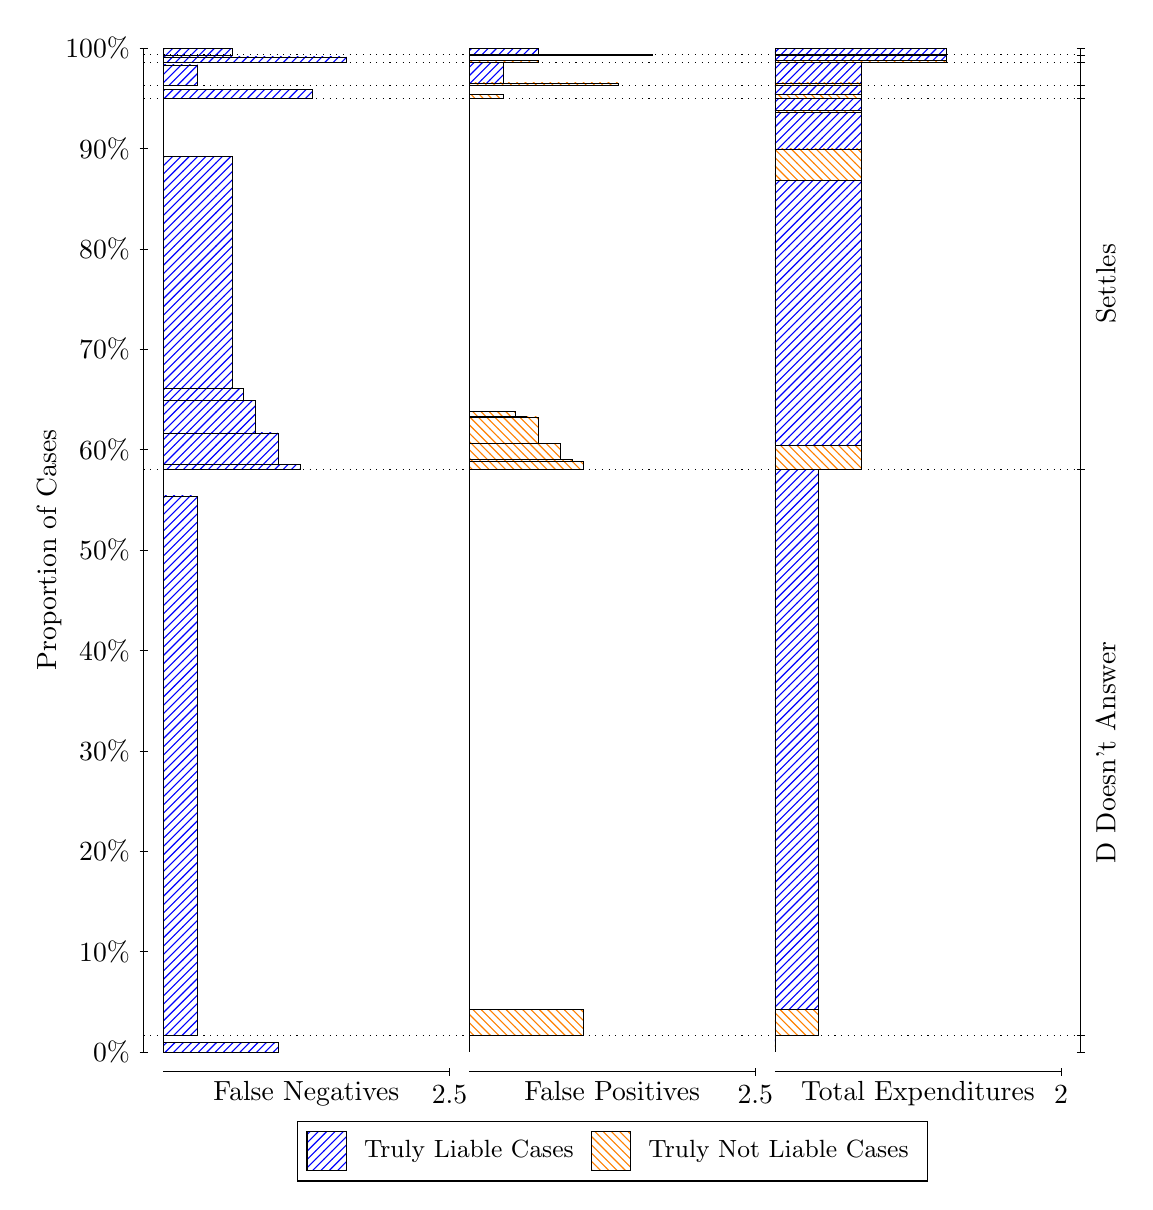
\begin{tikzpicture}
\draw[black, very thin] (1.5,1.75) -- (1.5,14.5);
\node[rotate=90, text=black, anchor=center] at (0.3, 8.125) {Proportion of Cases};
\draw[black, very thin] (1.45,1.75) -- (1.55,1.75);
\node[text=black, anchor=east] at (1.45, 1.75) {0\%};
\draw[black, very thin] (1.45,3.025) -- (1.55,3.025);
\node[text=black, anchor=east] at (1.45, 3.025) {10\%};
\draw[black, very thin] (1.45,4.3) -- (1.55,4.3);
\node[text=black, anchor=east] at (1.45, 4.3) {20\%};
\draw[black, very thin] (1.45,5.575) -- (1.55,5.575);
\node[text=black, anchor=east] at (1.45, 5.575) {30\%};
\draw[black, very thin] (1.45,6.85) -- (1.55,6.85);
\node[text=black, anchor=east] at (1.45, 6.85) {40\%};
\draw[black, very thin] (1.45,8.125) -- (1.55,8.125);
\node[text=black, anchor=east] at (1.45, 8.125) {50\%};
\draw[black, very thin] (1.45,9.4) -- (1.55,9.4);
\node[text=black, anchor=east] at (1.45, 9.4) {60\%};
\draw[black, very thin] (1.45,10.675) -- (1.55,10.675);
\node[text=black, anchor=east] at (1.45, 10.675) {70\%};
\draw[black, very thin] (1.45,11.95) -- (1.55,11.95);
\node[text=black, anchor=east] at (1.45, 11.95) {80\%};
\draw[black, very thin] (1.45,13.225) -- (1.55,13.225);
\node[text=black, anchor=east] at (1.45, 13.225) {90\%};
\draw[black, very thin] (1.45,14.5) -- (1.55,14.5);
\node[text=black, anchor=east] at (1.45, 14.5) {100\%};

\draw[black, very thin] (13.4,1.75) -- (13.4,14.5);
\draw[black, very thin] (13.35,1.75) -- (13.45,1.75);
\node[anchor=west] at (13.35, 1.75) {};
\draw[black, very thin] (13.35,1.9584) -- (13.45,1.9584);
\node[anchor=west] at (13.35, 1.9584) {};
\draw[black, very thin] (13.35,9.1465) -- (13.45,9.1465);
\node[anchor=west] at (13.35, 9.1465) {};
\draw[black, very thin] (13.35,13.862) -- (13.45,13.862);
\node[anchor=west] at (13.35, 13.862) {};
\draw[black, very thin] (13.35,14.023) -- (13.45,14.023);
\node[anchor=west] at (13.35, 14.023) {};
\draw[black, very thin] (13.35,14.321) -- (13.45,14.321);
\node[anchor=west] at (13.35, 14.321) {};
\draw[black, very thin] (13.35,14.414) -- (13.45,14.414);
\node[anchor=west] at (13.35, 14.414) {};
\draw[black, very thin] (13.35,14.5) -- (13.45,14.5);
\node[anchor=west] at (13.35, 14.5) {};

\draw[black, very thin, pattern color=blue, pattern=north east lines] (1.75,1.75) rectangle (3.2033,1.8678);
\draw[black, very thin, pattern color=orange, pattern=north west lines] (1.75,1.8678) rectangle (1.75,1.9584);
\draw[black, very thin, pattern color=blue, pattern=north east lines] (1.75,1.9584) rectangle (2.186,8.8129);
\draw[black, very thin, pattern color=orange, pattern=north west lines] (1.75,8.8129) rectangle (1.75,9.1465);
\draw[black, very thin, pattern color=blue, pattern=north east lines] (1.75,9.1465) rectangle (3.494,9.212);
\draw[black, very thin, pattern color=blue, pattern=north east lines] (1.75,9.212) rectangle (3.3487,9.2162);
\draw[black, very thin, pattern color=blue, pattern=north east lines] (1.75,9.2162) rectangle (3.2033,9.6117);
\draw[black, very thin, pattern color=blue, pattern=north east lines] (1.75,9.6117) rectangle (2.9127,10.024);
\draw[black, very thin, pattern color=blue, pattern=north east lines] (1.75,10.024) rectangle (2.7673,10.175);
\draw[black, very thin, pattern color=blue, pattern=north east lines] (1.75,10.175) rectangle (2.622,13.128);
\draw[black, very thin, pattern color=orange, pattern=north west lines] (1.75,13.128) rectangle (1.75,13.862);
\draw[black, very thin, pattern color=blue, pattern=north east lines] (1.75,13.862) rectangle (3.6393,13.974);
\draw[black, very thin, pattern color=orange, pattern=north west lines] (1.75,13.974) rectangle (1.75,14.023);
\draw[black, very thin, pattern color=blue, pattern=north east lines] (1.75,14.023) rectangle (2.186,14.287);
\draw[black, very thin, pattern color=orange, pattern=north west lines] (1.75,14.287) rectangle (1.75,14.321);
\draw[black, very thin, pattern color=blue, pattern=north east lines] (1.75,14.321) rectangle (4.0753,14.388);
\draw[black, very thin, pattern color=orange, pattern=north west lines] (1.75,14.388) rectangle (1.75,14.414);
\draw[black, very thin, pattern color=blue, pattern=north east lines] (1.75,14.414) rectangle (2.622,14.493);
\draw[black, very thin, pattern color=orange, pattern=north west lines] (1.75,14.493) rectangle (1.75,14.5);
\draw[black, very thin, pattern color=orange, pattern=north west lines] (5.6333,1.75) rectangle (5.6333,1.8406);
\draw[black, very thin, pattern color=blue, pattern=north east lines] (5.6333,1.8406) rectangle (5.6333,1.9584);
\draw[black, very thin, pattern color=orange, pattern=north west lines] (5.6333,1.9584) rectangle (7.0867,2.292);
\draw[black, very thin, pattern color=blue, pattern=north east lines] (5.6333,2.292) rectangle (5.6333,9.1465);
\draw[black, very thin, pattern color=orange, pattern=north west lines] (5.6333,9.1465) rectangle (7.0867,9.2474);
\draw[black, very thin, pattern color=orange, pattern=north west lines] (5.6333,9.2474) rectangle (6.9413,9.2742);
\draw[black, very thin, pattern color=orange, pattern=north west lines] (5.6333,9.2742) rectangle (6.796,9.4834);
\draw[black, very thin, pattern color=orange, pattern=north west lines] (5.6333,9.4834) rectangle (6.5053,9.8169);
\draw[black, very thin, pattern color=orange, pattern=north west lines] (5.6333,9.8169) rectangle (6.36,9.8197);
\draw[black, very thin, pattern color=orange, pattern=north west lines] (5.6333,9.8197) rectangle (6.2147,9.881);
\draw[black, very thin, pattern color=blue, pattern=north east lines] (5.6333,9.881) rectangle (5.6333,13.862);
\draw[black, very thin, pattern color=orange, pattern=north west lines] (5.6333,13.862) rectangle (6.0693,13.911);
\draw[black, very thin, pattern color=blue, pattern=north east lines] (5.6333,13.911) rectangle (5.6333,14.023);
\draw[black, very thin, pattern color=orange, pattern=north west lines] (5.6333,14.023) rectangle (7.5227,14.057);
\draw[black, very thin, pattern color=blue, pattern=north east lines] (5.6333,14.057) rectangle (6.0693,14.321);
\draw[black, very thin, pattern color=orange, pattern=north west lines] (5.6333,14.321) rectangle (6.5053,14.347);
\draw[black, very thin, pattern color=blue, pattern=north east lines] (5.6333,14.347) rectangle (5.6333,14.414);
\draw[black, very thin, pattern color=orange, pattern=north west lines] (5.6333,14.414) rectangle (7.9587,14.422);
\draw[black, very thin, pattern color=blue, pattern=north east lines] (5.6333,14.422) rectangle (6.5053,14.5);
\draw[black, very thin, pattern color=orange, pattern=north west lines] (9.5167,1.75) rectangle (9.5167,1.8406);
\draw[black, very thin, pattern color=blue, pattern=north east lines] (9.5167,1.8406) rectangle (9.5167,1.9584);
\draw[black, very thin, pattern color=orange, pattern=north west lines] (9.5167,1.9584) rectangle (10.062,2.292);
\draw[black, very thin, pattern color=blue, pattern=north east lines] (9.5167,2.292) rectangle (10.062,9.1465);
\draw[black, very thin, pattern color=orange, pattern=north west lines] (9.5167,9.1465) rectangle (10.607,9.4567);
\draw[black, very thin, pattern color=blue, pattern=north east lines] (9.5167,9.4567) rectangle (10.607,12.822);
\draw[black, very thin, pattern color=orange, pattern=north west lines] (9.5167,12.822) rectangle (10.607,13.22);
\draw[black, very thin, pattern color=blue, pattern=north east lines] (9.5167,13.22) rectangle (10.607,13.685);
\draw[black, very thin, pattern color=orange, pattern=north west lines] (9.5167,13.685) rectangle (10.607,13.712);
\draw[black, very thin, pattern color=blue, pattern=north east lines] (9.5167,13.712) rectangle (10.607,13.862);
\draw[black, very thin, pattern color=orange, pattern=north west lines] (9.5167,13.862) rectangle (10.607,13.911);
\draw[black, very thin, pattern color=blue, pattern=north east lines] (9.5167,13.911) rectangle (10.607,14.023);
\draw[black, very thin, pattern color=orange, pattern=north west lines] (9.5167,14.023) rectangle (10.607,14.057);
\draw[black, very thin, pattern color=blue, pattern=north east lines] (9.5167,14.057) rectangle (10.607,14.321);
\draw[black, very thin, pattern color=orange, pattern=north west lines] (9.5167,14.321) rectangle (11.697,14.347);
\draw[black, very thin, pattern color=blue, pattern=north east lines] (9.5167,14.347) rectangle (11.697,14.414);
\draw[black, very thin, pattern color=orange, pattern=north west lines] (9.5167,14.414) rectangle (11.697,14.422);
\draw[black, very thin, pattern color=blue, pattern=north east lines] (9.5167,14.422) rectangle (11.697,14.5);
\draw[black, dotted] (1.5,1.9584) -- (13.4,1.9584);
\draw[black, dotted] (1.5,9.1465) -- (13.4,9.1465);
\draw[black, dotted] (1.5,13.862) -- (13.4,13.862);
\draw[black, dotted] (1.5,14.023) -- (13.4,14.023);
\draw[black, dotted] (1.5,14.321) -- (13.4,14.321);
\draw[black, dotted] (1.5,14.414) -- (13.4,14.414);
\draw[black, very thin] (1.75,1.5) -- (5.3833,1.5);
\node[text=black, anchor=north] at (3.5667, 1.5) {False Negatives};
\draw[black, very thin] (5.3833,1.45) -- (5.3833,1.55);
\node[text=black, anchor=north] at (5.3833, 1.45) {2.5};

\draw[black, very thin] (5.6333,1.5) -- (9.2667,1.5);
\node[text=black, anchor=north] at (7.45, 1.5) {False Positives};
\draw[black, very thin] (9.2667,1.45) -- (9.2667,1.55);
\node[text=black, anchor=north] at (9.2667, 1.45) {2.5};

\draw[black, very thin] (9.5167,1.5) -- (13.15,1.5);
\node[text=black, anchor=north] at (11.333, 1.5) {Total Expenditures};
\draw[black, very thin] (13.15,1.45) -- (13.15,1.55);
\node[text=black, anchor=north] at (13.15, 1.45) {2};


\node[text=black, centered, rotate=90] at (13.72, 5.5524) {D Doesn't Answer};
\node[text=black, centered, rotate=90] at (13.72, 11.504) {Settles};





\draw (7.449999999999999,1.5) node[draw=none] (baseCoordinate) {};
\begin{scope}[align=center]
        \matrix[scale=0.5, draw=black, below=0.5cm of baseCoordinate, nodes={draw}, column sep=0.1cm]{
            \node[rectangle, draw, minimum width=0.5cm, minimum height=0.5cm, pattern color=blue, pattern=north east lines] {}; &
            \node[draw=none, font=\small, text=black] (B) {Truly Liable Cases}; &
            \node[rectangle, draw, minimum width=0.5cm, minimum height=0.5cm, pattern color=orange, pattern=north west lines] {}; &
            \node[draw=none, font=\small, text=black] (B) {Truly Not Liable Cases}; \\
            };
\end{scope}

\end{tikzpicture}
\end{document}